\documentclass{article}

\PassOptionsToPackage{numbers, compress}{natbib}
\usepackage{nips_2017}
\usepackage{listings}
\usepackage{textcomp}
\usepackage[usenames,dvipsnames,svgnames]{xcolor}
\usepackage{graphicx}
\usepackage[subrefformat=parens]{subcaption}

\newcommand{\expr}[0]{\texttt{<expr>}}
\newcommand{\address}[0]{\texttt{<address>}}

%!TEX root = ./main.tex

\lstset{
  basicstyle=\ttfamily\scriptsize,
  columns=fullflexible,
  keepspaces=true,
  upquote=true,
  % Define . and % and @ as letters to include them in keywords.
  alsoletter={\.,\%,\#, \@, \?, \/},
  % First type of keywords.
  morekeywords=[1]{function, if, else, end, for, begin, in, const, struct, using, return},
  keywordstyle=[1]\textcolor{Brown},
  % Second type of keywords.
  morekeywords=[2]{\@gen, \@rand, \@param, \@input, \@output, \@tf_function, \@call, \@read, \@tf_call},
  keywordstyle=[2]\textcolor{RoyalBlue},
  % Add strings
  showstringspaces=False,
  %stringstyle=\ttfamily\color{NavyBlue},
  %stringstyle=\ttfamily\color{Purple},
  %morestring=[b]{"},
  %morestring=[b]{'},
  % l is for line comment
  morecomment=[l]{\#},
  commentstyle=\color{Gray}\ttfamily,
  escapeinside={<@}{@>}
}

\newcommand{\addr}[1]{\textcolor{DarkGreen}{#1}}


\title{Customizable deep learning and Monte Carlo for probabilistic inference using probabilistic programs}

\begin{document}

\maketitle

\begin{abstract}

\end{abstract}

\section{Introduction}

Contributions:
\begin{enumerate}
\item A universal probabilistic programming system that combines programmable Monte Carlo inference with scalable and customizable deep learning.
\item We show how to express data-driven proposals as probabilistic programs that embed custom deep neural networks, and how to train these proposals on data simulated from a generative model.
\item We show how a simple combination of model-based Monte Carlo and deep learning can improve upon pure deep learning based inference.
\end{enumerate}

\section{Background: Programmable Inference in GenLite}
GenLite \cite{TODO} is a flexible probabilistic programming language designed to support user-programmable inference.
This section provides a very brief introduction to GenLite.
GenLite is embedded in Julia \cite{TODO}.
In GenLite, users first express a probabilistic generative model as a \emph{generative function}, which is written in an embedded DSL that extends Julia functions with the ability to make traced random choies.
Then, users implement Monte Carlo inference algorithms for the model in Julia code, drawing heavily on GenLite's inference programming API, which provides core data structures and inference primitives that utilize the programmatic representation of the generative model.
User inference code is written at a higher level of abstraction than typical custom sampler implementations, which makes it more efficient to develop, maintain, and reason about.

In GenLite, a \emph{trace} is a Julia value (of type \texttt{Trace}) that contains a record of random choices made by some generative function.
Generative functions, which are declared with keyword \texttt{@gen function}, extend Julia with three language constructs:
\begin{enumerate}
\item \texttt{@rand(<expr>, <address>)}: Sample a random value (i.e. a `random choice') from probability distribution \expr{}, where \address{} is a string or tuple of strings that specify a hierarchical name, or `address' for the random choice.
Record the random choice in the trace at the given address.
\item \texttt{@call(<expr>, <address>)}: Invoke a generative function given by \expr{}, and record the resulting trace for the invoked function under address \address{} in the current trace.
\item \texttt{@read(<address>)}: If an input trace is provided, read the value in the input trace at the given \address{}.
\end{enumerate}

Note that generative functions can contain arbitrary Julia code.
Figure~\ref{fig:model-code-figure} shows a generative function that only exercises the \texttt{@rand} keyword.

\subsection{Using generative functions to define proposal distributions}
Like probabilistic models, we represent proposals as probabilistic programs.
Proposal programs can be used in importance sampling, sequential Monte Carlo, and Markov chain Monte Carlo.
Proposal programs can include latent variables.

\begin{lstlisting}[basicstyle=\ttfamily\small]
(new_trace::Trace, new_score::Float64, alpha::Float64, val) = mh4(
        model::GenerativeFunction, model_args::Tuple,
        forward::GenerativeFunction, forward_args::Tuple,
        backward::GenerativeFunction, backward_args::Tuple,
        transform::TraceTransform, transform_args::Tuple,
        prev_trace::Trace, prev_score::Float64)
\end{lstlisting}


\subsection{Training proposal distributions on simulated data}
Proposal programs can be used on simulated data (cite the `probabilitsic programs as proposals' research).
Proposal programs can be trained for use as importance distributions or MCMC proposals.
Show the math for training (KL divergence and maximum likelihood).
Discuss static parameters.

\section{Scalable Deep Learning in GenLite using TensorFlow}
We extend GenLite with a \texttt{tf\_function} and \texttt{tf\_call} language constructs.
The \texttt{tf\_function} keyword is used to define \emph{GenLite TensorFlow functions}, which are functional TensorFlow computations with declared inputs, trainable parameters, and an output.
Discuss the reverse-mode AD integration.
Discuss vectorized (batched) training.

\begin{figure}[h]
\centering
    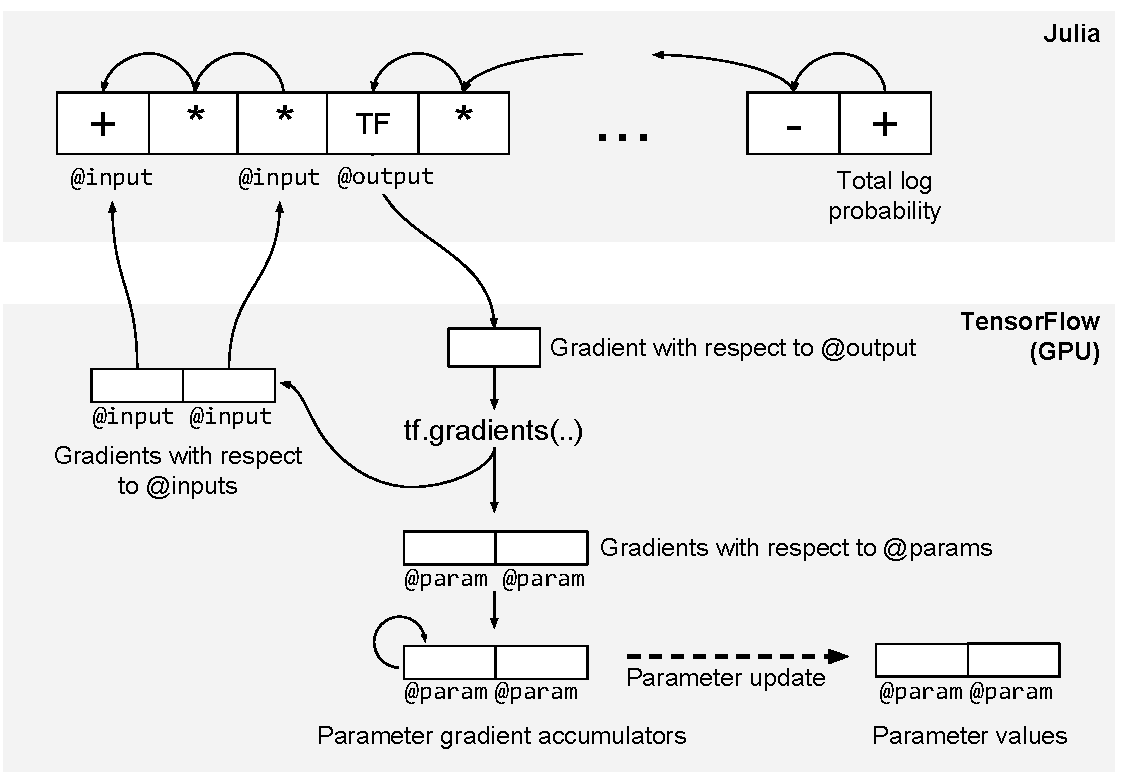
\includegraphics[width=0.7\textwidth]{images/tf-integration-schematic.pdf}
    \caption{
Reverse-mode AD in GenLite interoperates with `GenLite TensorFlow functions', which are blocks of functional TensorFlow (TF) code with inputs (corresponding to TF placeholders), trainable parameters (corresponding to TF variables), and an output, that are invoked by GenLite generative functions.
Each invocation of a TF function produces a single element on GenLite's reverse-mode AD tape.
During the backward pass (solid lines), we receive the gradient with respect to the output (\texttt{@output}) of the TF function; TF is used to compute the gradients with respect to inputs (\texttt{@input}) and parameters (\texttt{@params}).
The gradients with respect to the parameters are accumulated across multiple backward passes, until an parameter update is performed.
A parameter update (dashed line) changes the parameter values using the accumulated gradient (in addition to state of the update operation itself), and resets the gradient accumulators to zero.
Parameter updates are TF computations that are defined by the user separately from the TF function itself.
}
    \label{fig:tf-integration-schematic}
\end{figure}

\section{Combining Monte Carlo Inference and Deep Learning Proposals}
Because GenLite provides programmable inference, we can combine deep neural network proposals with other Monte Carlo strategies, like random walk moves, for refining a hypothesis.

\begin{figure}[t]
\begin{minipage}[t]{0.5\textwidth}
\begin{lstlisting}
using Cairo, ImageMagick, ImageFiltering
..

function render(glyph::Glyph)
  canvas = CairoRGBSurface(width, height)
  cc = CairoContext(canvas)
  Cairo.save(cc)

  # set background color to white
  Cairo.set_source_rgb(cc, 1.0, 1.0, 1.0)
  Cairo.rectangle(cc, 0.0, 0.0, width, height)
  Cairo.fill(cc)
  Cairo.restore(cc)
  Cairo.save(cc)

  # write the letter
  fontface = "Sans $(glyph.fontsize)"
  Cairo.set_font_face(cc, fontface)
  Cairo.text(cc, glyph.x, glyph.y, glyph.letter,
             angle=glyph.angle)

  return convert_to_png_blob(canvas)
end
\end{lstlisting}
\end{minipage}%
\begin{minipage}[t]{0.5\textwidth}
\begin{lstlisting}
model = @gen function()
  # prior
  x = width * @rand(uniform_cont(0, 1), <@\addr{"x"}@>)
  y = height * @rand(uniform_cont(0, 1), <@\addr{"y"}@>)
  size = @rand(uniform_cont(0, 1), <@\addr{"size"}@>)
  letter_id = @rand(uniform_disc(1, 3), <@\addr{"letter"}@>)
  letter = ["A", "B", "C"][letter_id]
  angle = 45 * @rand(uniform_cont(-1, 1), <@\addr{"angle"}@>)
  fontsize = scale_size(min_size, max_size, size)
  glyph = Glyph(x, y, angle, fontsize, letter)

  # render to png bytes
  image_png = render(glyph)

  # add Gaussian blur
  blur_width = 3
  blurred_png = imfilter(image_png,
                  Kernel.gaussian(blur_width))

  # add noise
  matrix = convert(Matrix{Float64}, blurred_png)
  @rand(speckle_noise(matrix, 0.1), <@\addr{"image"}@>)
end
\end{lstlisting}
\end{minipage}
\caption{Generative function for a generative model of blurry images that contain a single letter at a random location, rotation, and size. Addresses of random choices are shown in green.}
\label{fig:model-code-figure}
\end{figure}

\begin{figure}[t]
\begin{minipage}[t]{0.5\textwidth}
\begin{lstlisting}
using GenLiteTF
using TensorFlow
tf = TensorFlow

num_input = width * height
num_output = 11

function conv2d(x, W)
  tf.nn.conv2d(x, W, [1, 1, 1, 1], "SAME")
end

function max_pool_2x2(x)
  tf.nn.max_pool(x, [1, 2, 2, 1], [1, 2, 2, 1], "SAME")
end

function initial_weight(shape)
  randn(Float32, shape...) * 0.001f0
end

function initial_bias(shape)
  fill(0.1f0, shape...)
end

network = @tf_function begin

  # input image (N, 56 * 56)
  @input image_flat Float32 [-1, num_input]
  image = tf.reshape(image_flat, [-1, width, height, 1])

  # convolution + max-pooling (N, 28, 28, 32)
  @param W_conv1 initial_weight([5, 5, 1, 32])
  @param b_conv1 initial_bias([32])
  h_conv1 = tf.nn.relu(conv2d(image, W_conv1) + b_conv1)
  h_pool1 = max_pool_2x2(h_conv1)

  # convolution + max-pooling (N, 14, 14, 32)
  @param W_conv2 initial_weight([5, 5, 32, 32])
  @param b_conv2 initial_bias([32])
  h_conv2 = tf.nn.relu(conv2d(h_pool1, W_conv2) + b_conv2)
  h_pool2 = max_pool_2x2(h_conv2)
  h_pool2_flat = tf.reshape(h_pool2, [-1, 14 * 14 * 32])

  # convolution + max-pooling (N, 7, 7, 64)
  @param W_conv3 initial_weight([5, 5, 32, 64])
  @param b_conv3 initial_bias([64])
  h_conv3 = tf.nn.relu(conv2d(h_pool2, W_conv3) + b_conv3)
  h_pool3 = max_pool_2x2(h_conv3)
  h_pool3_flat = tf.reshape(h_pool3, [-1, 7 * 7 * 64])

  # fully connected layer (N, 1024)
  @param W_fc1 initial_weight([7 * 7 * 64, 1024])
  @param b_fc1 initial_bias([1024])
  h_fc1 = tf.nn.relu(h_pool3_flat * W_fc1 + b_fc1)

  # output layer (N, 11)
  @param W_fc2 initial_weight([1024, num_output])
  @param b_fc2 initial_bias([num_output])
  @output Float32 (tf.matmul(h_fc1, W_fc2) + b_fc2)
end

\end{lstlisting}
\end{minipage}%
\hfill
\begin{minipage}[t]{0.4\textwidth}
\begin{lstlisting}
predict = @gen function (outputs)

  # predict the x-coordinate
  x_mu = outputs[1]
  x_std = exp(outputs[2])
  @rand(normal(x_mu, x_std), <@\addr{"x"}@>)

  # predict the y-coordinate
  y_mu = outputs[3]
  y_std = exp(outputs[4])
  @rand(normal(y_mu, y_std), <@\addr{"y"}@>)

  # predict the rotation
  r_mu = exp(outputs[5])
  r_std = exp(outputs[6])
  @rand(normal(r_mu, r_std), <@\addr{"angle"}@>)

  # predict the size 
  size_alpha = exp(outputs[7])
  size_beta = exp(outputs[8])
  @rand(Gen.beta(size_alpha, size_beta), <@\addr{"size"}@>)
  
  # predict the identity of the letter
  log_letter_dist = outputs[9:end]
  letter_dist = exp.(log_letter_dist)
  letter_dist = letter_dist / sum(letter_dist)
  @rand(categorical(letter_dist), <@\addr{"letter"}@>)
end

proposal = @gen function ()

  # get image from input trace
  image = zeros(1, num_input)
  image[1,:] = @read(<@\addr{"image"}@>)[:]

  # run inference network
  outputs = @tf_call(network(image))

  # make prediction given inference network outputs
  @splice(predict(outputs[1,:]))
end

proposal_batch = @gen function (batch_size)

  # get images from input trace
  images = zeros(Float32, batch_size, num_input)
  for i=1:batch_size
    images[i,:] = @read((<@\addr{"\$i"}@>, <@\addr{"image"}@>))[:]
  end

  # run inference network in batch
  outputs = @tf_call(network(images))
  
  # make prediction for each image
  for i=1:batch_size
    @call(predict(outputs[i,:]), <@\addr{"\$i"}@>)
  end
end
\end{lstlisting}
\end{minipage}
\caption{
A GenLite TensorFlow (TF) function (\texttt{network}) that is invoked by a generative function (\texttt{proposal}) that implements a data-driven proposal for the model of Figure~\ref{fig:model-code-figure}.
GenLite TF functions are identified by a \texttt{@tf\_function} keyword.
The user declares inputs (\texttt{@input}, corresponding to TF placeholders), parameters (\texttt{@param}, corresponding to TF variables) and an output tensor (\texttt{@output}).
The rest of the code inside the \texttt{@tf\_function} block is regular TensorFlow code, using the TensorFlow.jl Julia wrapper \cite{?} around the TensorFlow C API.
The proposal reads the image from an input trace, runs the network, and then uses its output to parametrize distributions on the latent variables in the model.
To scalably train the network on GPU hardware, we also implement a batched variant of the proposal program, which reads from and writes to vector-shaped traces.
The batched and unbatched variants of the reuse both the TensorFlow and probabilistic prediction code.
}
\label{fig:proposal-code-figure}
\end{figure}


%x = width * @rand(uniform_cont(0, 1), <@\addr{"x"}@>)

\begin{figure}[t]
\begin{subfigure}[b]{0.6\textwidth}
\begin{lstlisting}
grads_and_vars = []
zero_grad_ops = []
for (param_name) in <@\infr{get\_param\_names}@>(network)
  grad = tf.negative(<@\infr{get\_param\_grad}@>(network, param_name))
  var = <@\infr{get\_param\_var}@>(network, param_name)
  push!(grads_and_vars, (grad, var))
  push!(zero_grad_ops, <@\infr{get\_zero\_grad\_op}@>(network, param_name))
end
optimizer = tf.train.AdamOptimizer(1e-4)
network_update = tf.group(
  tf.train.apply_gradients(optimizer, grads_and_vars),
  zero_grad_ops...)
\end{lstlisting}
\caption{Defining the update to the TensorFlow parameters}
\end{subfigure}%
\begin{subfigure}[b]{0.4\textwidth}
\begin{lstlisting}
num_train = 100000
traces = Vector{Trace}(num_train)
for i=1:num_train
  (traces[i], _, _) = <@\infr{simulate}@>(model, ())
end
\end{lstlisting}
\caption{Simulating training data from the model}
\end{subfigure}
\begin{subfigure}[b]{\textwidth}
\begin{lstlisting}
tf.run(get_tf_session(), tf.global_variables_initializer())
batch_size = 100
for iter=1:num_iter
  batch_idx = randperm(num_train)[1:batch_size]
  traces = all_traces[batch_idx]
  vector_trace = <@\infr{vectorize}@>(traces)
  (total_score, _) = <@\infr{backprop}@>(proposal_batch, (batch_size,), vector_trace, vector_trace)
  tf.run(get_tf_session(), network_update)
  score = total_score / batch_size
end
\end{lstlisting}
\caption{Training the proposal on simulated data}
\end{subfigure}
\caption{
Julia code for training the data-driven proposal distribution of Figure~\ref{fig:proposal-code-figure} to propose the latent variables of the generative model (\texttt{model}) of Figure~\ref{fig:model-code-figure} given an observed image.
In (a), we define an TensorFlow (TF) operation (\texttt{network\_update}) that will be used to update the parameters of the TF function \texttt{network} (defined in Figure~\ref{fig:proposal-code-figure}.
We define the operation in terms of the parameter value variables and parameter gradient accumulator variables that are accessible with GenLite API functions \texttt{get\_param\_var} and \texttt{get\_param\_grad}, respectively.
The update applies an ADAM update to all of the parameters and then zeros-out the gradient accumulators.
Next, in (b), we generate training data by sampling traces from the model.
These traces contain both the observed image (at address \texttt{"image"}) and all of the latent variables (\texttt{"x"}, \texttt{"y"}, ..).
Finally, in (c), we perform training using batches.
We group a set of traces of \texttt{model} into a vector-shaped trace using \texttt{vectorize}.
We then run \texttt{backprop} on the generative function \texttt{proposal\_batch}, where we use \texttt{vector\_trace} as both the input trace (from which the image is read) and the output trace (which contains the ground truth latent variables for the corresponding image).
GenLite API functions are shown in purple.
}
\label{fig:training-code-figure}
\end{figure}


\section{Example}

\begin{figure}[h]
\centering
    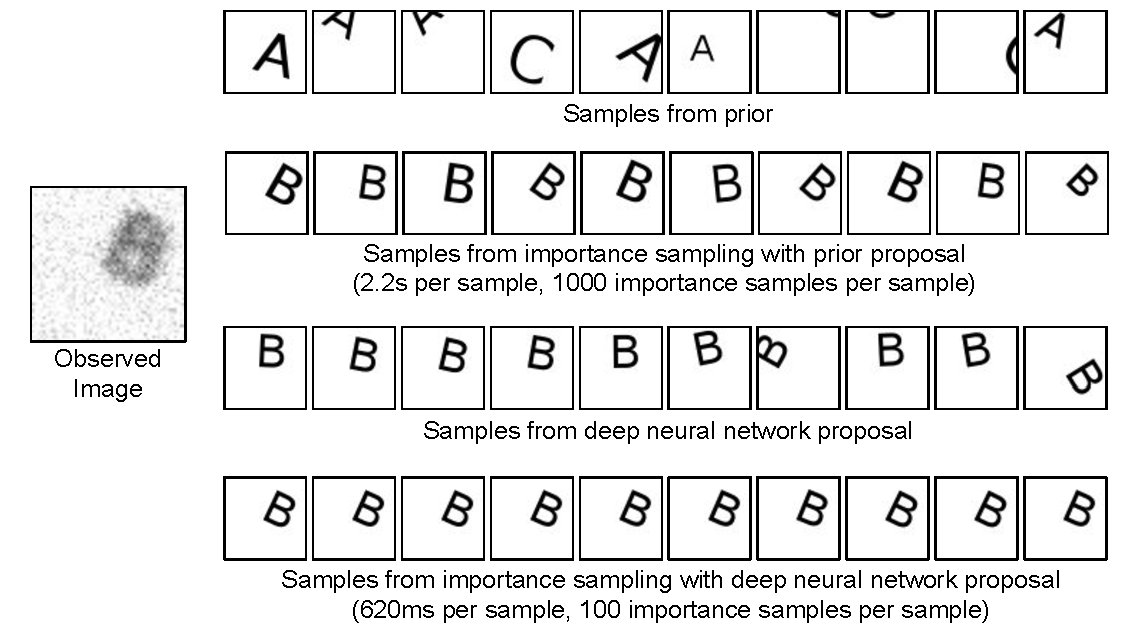
\includegraphics[width=1.0\textwidth]{images/deep-neural-network-is.pdf}
    \caption{
Inference in the generative model of Figure~\ref{fig:model-code-figure} using a combination of deep learning and model-based Monte Carlo.
On the left is the observed image, followed by a set of 10 of latent images sampled from the trained deep neural network proposal (\texttt{proposal} in Figure~\ref{fig:proposal-code-figure}), and a set of 10 latent images sampled using importance sampling, with the trained deep neural network proposal as the importance distribution.
The deep neural network was trained on traces and images jointly sampled from the generative model, using ADAM with 170,000 iterations, each with batch size 100.
The deep neural network proposal is uncertain about the location and orientiation of the letter.
Augmenting the neural network with model-based importance sampling gives more accurate inferences.
}
    \label{fig:example-results}
\end{figure}

See Figure~\ref{fig:model-code-figure}.


\section{Related Work}
Guide programs in Pyro,
Using probabilisic programs as proposals,
Edward,
Stuart Russell work on block neural proposals,
Tuan An Le's work on univeral compiled inference,
Wake sleep,
Helmholtz machines,
VAE,
Stochastic inverses

\subsubsection*{Acknowledgments}
This research was supported by DARPA (PPAML program, contract number FA8750-14-2-0004), IARPA (under research contract 2015-15061000003), the Office of Naval Research (under research contract N000141310333), the Army Research Office (under agreement number W911NF-13-1-0212), and gifts from Analog Devices and Google.
This research was conducted with Government support under and awarded by DoD, Air Force Office of Scientific Research, National Defense Science and Engineering Graduate (NDSEG) Fellowship, 32 CFR 168a.

\bibliographystyle{unsrtnat}
\bibliography{references}

\end{document}
